\newpage
\section{System call}

% Funzioni e system call
\subsection{Funzioni e system call}

Se prendiamo un funzionamento più semplice del comando "ls" potrebbe essere:

\begin{lstlisting}
#include "apue.h"
#include <dirent.h>

int
main(int argc, char *argv[])
{
	DIR				*dp;
	struct dirent	*dirp;

	if (argc != 2)
		err_quit("usage: ls1 directory_name");

	if ((dp = opendir(argv[1])) == NULL)
		err_sys("can't open %s", argv[1]);
	while ((dirp = readdir(dp)) != NULL)
		printf("%s\n", dirp->d_name);

	closedir(dp);
	exit(0);
}
\end{lstlisting}


dove abbiamo che:

\begin{itemize}
	\item \hl{DIR}: struttura dati
	\item \hl{struct dirent}: \textbf{tipo struttura} che contiene al suo interno diversi tipi di variabili. 
	
		Per capire se è una funzione di sistema lanciamo:
		
\begin{lstlisting}
grep -rw "struct dirent" $INC
\end{lstlisting}
		
		seguiamo il percorso:
		
\begin{lstlisting}
/Applications/Xcode.app/Contents/Developer/Platforms/MacOSX.platform/Developer/SDKs/MacOSX.sdk/usr/include//sys/dirent.h:struct dirent {
\end{lstlisting}
		
\begin{lstlisting}
#ifndef _SYS_DIRENT_H
#define _SYS_DIRENT_H

#include <sys/_types.h>
#include <sys/cdefs.h>

#include <sys/_types/_ino_t.h>


#define __DARWIN_MAXNAMLEN      255

#pragma pack(4)

#if !__DARWIN_64_BIT_INO_T
struct dirent {
	ino_t d_ino;                    /* file number of entry */
	__uint16_t d_reclen;            /* length of this record */
	__uint8_t  d_type;              /* file type, see below */
	__uint8_t  d_namlen;            /* length of string in d_name */
	char d_name[__DARWIN_MAXNAMLEN + 1];    /* name must be no longer than this */
};
#endif /* !__DARWIN_64_BIT_INO_T */

#pragma pack()

#define __DARWIN_MAXPATHLEN     1024

#define __DARWIN_STRUCT_DIRENTRY { \
	__uint64_t  d_ino;      /* file number of entry */ \
	__uint64_t  d_seekoff;  /* seek offset (optional, used by servers) */ \
	__uint16_t  d_reclen;   /* length of this record */ \
	__uint16_t  d_namlen;   /* length of string in d_name */ \
	__uint8_t   d_type;     /* file type, see below */ \
	char      d_name[__DARWIN_MAXPATHLEN]; /* entry name (up to MAXPATHLEN bytes) */ \
}

#if __DARWIN_64_BIT_INO_T
struct dirent __DARWIN_STRUCT_DIRENTRY;
#endif /* __DARWIN_64_BIT_INO_T */



#if !defined(_POSIX_C_SOURCE) || defined(_DARWIN_C_SOURCE)
#define d_fileno        d_ino           /* backward compatibility */
#define MAXNAMLEN       __DARWIN_MAXNAMLEN
/*
 * File types
 */
#define DT_UNKNOWN       0
#define DT_FIFO          1
#define DT_CHR           2
#define DT_DIR           4
#define DT_BLK           6
#define DT_REG           8
#define DT_LNK          10
#define DT_SOCK         12
#define DT_WHT          14

/*
 * Convert between stat structure types and directory types.
 */
#define IFTODT(mode)    (((mode) & 0170000) >> 12)
#define DTTOIF(dirtype) ((dirtype) << 12)
#endif


#endif /* _SYS_DIRENT_H  */
\end{lstlisting}

		dove vediamo che se la variabile "\_\_DARWIN\_64\_BIT\_INO\_T" è stata definita avremo che la struttura di struct dirent è:
		
\begin{lstlisting}
#define __DARWIN_STRUCT_DIRENTRY { \
	__uint64_t  d_ino;      /* file number of entry */ \
	__uint64_t  d_seekoff;  /* seek offset (optional, used by servers) */ \
	__uint16_t  d_reclen;   /* length of this record */ \
	__uint16_t  d_namlen;   /* length of string in d_name */ \
	__uint8_t   d_type;     /* file type, see below */ \
	char      d_name[__DARWIN_MAXPATHLEN]; /* entry name (up to MAXPATHLEN bytes) */ \
}

#if __DARWIN_64_BIT_INO_T
struct dirent __DARWIN_STRUCT_DIRENTRY;
#endif /* __DARWIN_64_BIT_INO_T */
\end{lstlisting}

		
	\item \hl{if}: esegue un controllo sugli args. Notiamo che "err\_quit" non è una funzione di sistema da:
	
\begin{lstlisting}
grep -rw "err_quit" $INC
\end{lstlisting}

		infatti non restituisce nulla. Deve allora essere una funzione di libreria create da noi quindi non presente nella directory standard.
		
		La funzione andrà a dare un messaggio di errore e poi esce dal programma.
		
		
	\item \hl{opendir}: serve ad aprire una directory andandola a caricare nella RAM. 
	
	\item \hl{while}: leggiamo la directory e la inseriamo nella struttura che poi sarà richiamata tramite:
	
\begin{lstlisting}
dirp->d_name
\end{lstlisting}

		dove "d\_name" è il nome dello slot in cui è contenuto il nome del file.
		
		
	\item \hl{exit}: restituisce l'exit code del programma
	
\end{itemize}


% Capire se una funzione è una system call
\subsection{Capire se una funzione è una system call}

Andiamo a \hl{vedere se e' una funzione o una system call tramite "man"}, lo si capisce tramite la dicitura in alto alla pagina del manuale:

	\begin{itemize}
		\item \textbf{Library Functions} Manual
		\item \textbf{System Calls} Manual
	\end{itemize}

Abbiamo anche \hl{esempi piu' particolari}, come fork, dove è indicata come system call ma in realtà le richiama ma in prima persona.


Potremo trovare i simboli di una libreria tramite:

\begin{lstlisting}
nm lib.a
\end{lstlisting}

che ci fa vedere, per ogni file oggetto, i simboli associati per ogni funzione.

Le system call le troveremo in "\$INC/sys/syscall.h"


% Numeri dei file descriptor
\subsection{Numeri dei file descriptor}

Prendiamo un esempio semplificato del comando "cat":

\begin{lstlisting}
#include "apue.h"

#define	BUFFSIZE	4096

int
main(void)
{
	int		n;
	char	buf[BUFFSIZE];

	while ((n = read(STDIN_FILENO, buf, BUFFSIZE)) > 0)
		if (write(STDOUT_FILENO, buf, n) != n)
			err_sys("write error");

	if (n < 0)
		err_sys("read error");

	exit(0);
}
\end{lstlisting}

\hl{ogni processo ha 3 file descriptor usati 0, 1, 2}.

\begin{itemize}
	\item \hl{BUFFSIZE}: macro di preprocessore
	\item \hl{read}: \textbf{system call} con parametri: 
	
		\begin{itemize}
			\item \textbf{STDIN\_FILENO}: file descriptor per dire da quale "numero di deve leggere" si vuole leggere. Cioè per leggere dal file indicato nello standard input
			\item \textbf{buf}: indirizzo dell'\textbf{inizio dell'array}
			\item \textbf{BUFFSIZE}: quando deve leggere
		\end{itemize}
		
		\hl{Restituisce il numero di char che ha letto}, dato che potrebbe leggere meno byte di quelli richiesti nel caso in cui il file ne contenga di meno. Ad ogni sua iterazione \hl{si ricorda la "posizione nel file"} che gli permette di non leggere sempre i primi n byte ma di rincominciare da dove ha lasciato.
	
	\item \hl{write}: richiede gli stessi valori di read tranne per \textbf{STDOUT\_FILENO} e \textbf{ritorna il numero byte effettivamente letti}
	\item 
\end{itemize}


per capire \hl{quanto vale STDIN\_FILENO}:


\begin{lstlisting}
$ grep -rw "STDIN_FILENO" $INC
/Applications/Xcode.app/Contents/Developer/Platforms/MacOSX.platform/Developer/SDKs/MacOSX.sdk/usr/include//unistd.h:#define	 STDIN_FILENO	0	/* standard input file descriptor */
/Applications/Xcode.app/Contents/Developer/Platforms/MacOSX.platform/Developer/SDKs/MacOSX.sdk/usr/include//asl.h: * asl_log_descriptor(c, m, ASL_LEVEL_NOTICE, STDIN_FILENO, ASL_LOG_DESCRIPTOR_READ);
\end{lstlisting}


Sappiamo che un processo per eseguire un programma, esegue prima una \hl{fork} e poi con \hl{exec} esegue il programma. Prima di eseguire la fork il \hl{child chiude il file 1} e quando fa una \hl{open}, la system call prenderà il file nel quale reindirizzare lo STDOUT e restituirà il numero 1.

Su questo sistema si base UINX infatti avviene anche con le pipe "|". Permette di creare programmi complessi unendo tanti piccoli programmi specializzati in un'unica funzione.

È molto importante capire che \hl{ i child ereditano i file descriptor dei parent} quindi non è necessario che il programma corrente faccia una open dei file descriptor.


% Meccanismi dei file
\subsection{Meccanismi dei file}

Un file è in insieme di meccanismi: 

\begin{itemize}
	\item \hl{apri}
	\item \hl{leggi}
	\item \hl{scrivi}
	\item \hl{chiudi}
\end{itemize}


Questi meccanismi sono applicabili a file, cartelle, stampanti ecc..., solo che per ogni "tipo" \hl{i 4 meccanismi si adeguano} a ciò che il caso particolare deve fare.


% Unbuffered I/O
\subsection{Unbuffered I/O}

Le system call rappresentano una barriera tra kernel e programmi, dove avremo rispettivamente \hl{due diverse modalita' di utilizzo}:

\begin{itemize}
	\item \textbf{kernel mode}: ha tutti i privilegi
	\item \textbf{user mode}: non può accedere a tutte le celle di memoria
\end{itemize}


Per \hl{ottimizzare la scrittura sulla memoria da parte del kernel si utilizza la libreria STDIOLIB} che incrementa le prestazioni dato che gestisce il passaggio di pacchetti con il kernel in modo da inviare dei pacchetti consistenti ogni tot e non piccoli pacchetti soni secondo. Per fare ciò usa un \hl{buffered i/o} che, una volta riempiti dei buffer, gli manda al kernel.


\begin{figure}[H]
\centering
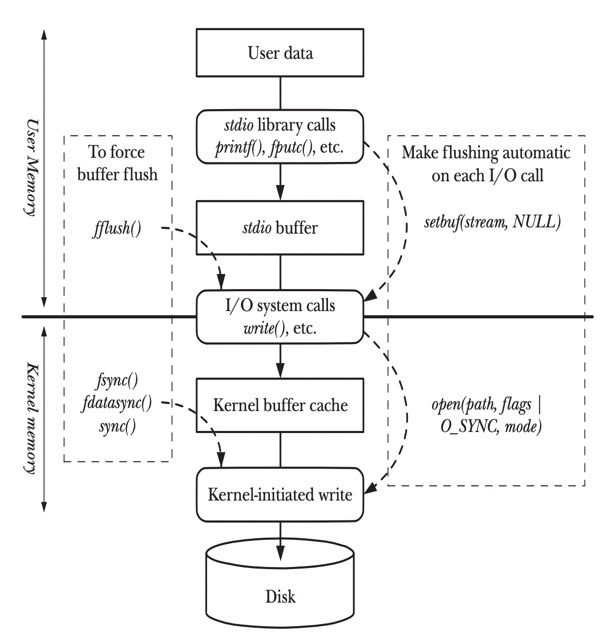
\includegraphics[scale=0.4]{unbuffio.jpeg}
\caption{Schema unbuffered I/O} 
\label{unbuffio}
\end{figure}




----
Prendiamo shell1.c che crea uno schell dal quale poter eseguire programmi:

\begin{lstlisting}
#include "apue.h"
#include <sys/wait.h>

int
main(void)
{
	char	buf[MAXLINE];	/* from apue.h */
	pid_t	pid;
	int		status;

	printf("%% ");	/* print prompt (printf requires %% to print %) */
	while (fgets(buf, MAXLINE, stdin) != NULL) {
		if (buf[strlen(buf) - 1] == '\n')
			buf[strlen(buf) - 1] = 0; /* replace newline with null */

		if ((pid = fork()) < 0) {
			err_sys("fork error");
		} else if (pid == 0) {		/* child */
			execlp(buf, buf, (char *)0);
			err_ret("couldn't execute: %s", buf);
			exit(127);
		}

		/* parent */
		if ((pid = waitpid(pid, &status, 0)) < 0)
			err_sys("waitpid error");
		printf("%% ");
	}
	exit(0);
}
\end{lstlisting}

avremo allora:

\begin{itemize}
	\item \hl{fgets}: funzione della \textbf{stdoutput che legge la riga} che dai prima di dare invio e la mette in un buffer, con argomenti:
	
		\begin{itemize}
			\item \textbf{MAXLINE}: proviene da una nostra libreria

\begin{lstlisting}
$ grep -rw "MAXLINE" include/
Binary file include//apue.h.gch matches
include//apue.h:#define	MAXLINE	4096			/* max line length */
\end{lstlisting}

			\item \textbf{stdin}: presente in stdiolib ed è una \textbf{struttura file che definisce uno standard input tramite un puntatore di un "file"}
		\end{itemize}

	\item \hl{if 1}: permette di avere un null dove prima avevamo \textbackslash n
	
	\item 
\end{itemize}